\newpage
\setcounter{page}{1}
\justifying
\noindent

\section{Navigation}
The first section of this paper will discuss in regards of navigation. The focused topic will be Inertial Navigation System (INS) and Enhanced Long Range Navigation system (E-LORAN). This section will include brief introduction, system mechanism, and real-life application for each type of navigation.

\subsection{Inertial Navigation System (INS)}
Inertia is the abilities of any physical object to maintain its transnational and rotational velocity unless external forces acted upon them. Inertial navigation  is a self-contained navigation which is used to track body position and orientation relative to its initial condition (point, orientation, and velocity) \cite{Woodman2007NumberNavigation}\cite{Ribbens2003AircraftInstruments}. This make INS as an autonomous system that  has no dependency on external information and does not radiates energy to space which allows its application in sea, airspace, and underground \cite{2018MiniatureUnit}. Inertial Measurement Unit (IMU) is the core of INS which normally consist of three orthogonal gyroscopes, three orthogonal accelerometer, and three orthogonal magnetometer (common in modern IMU) which measure 9 degree of freedom (DoF) movement \cite{Christ2014NavigationalSensors}. Figure \ref{fig:1} below shows both diagram of 6 DoF and 9 DoF IMUs.

\begin{figure}[!ht]
\centering
\begin{minipage}{.5\textwidth}
  \centering
  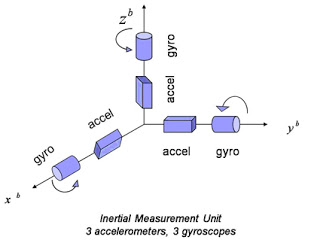
\includegraphics[height=0.7\linewidth]{Figures/imu_6dof.jpg}
  \captionof{figure}{Inertial Measurement Unit (IMU) with three orthogonal gyroscopes and accelerometer \cite{2021InertialTracking}.}
  \label{fig:IMU6DOF}
\end{minipage}%
\begin{minipage}{.5\textwidth}
  \centering
  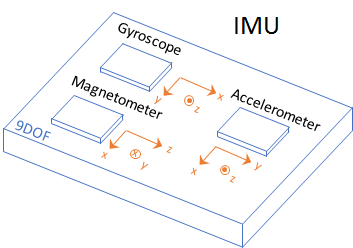
\includegraphics[height=0.7\linewidth]{Figures/imu_diagram.png}
  \captionof{figure}{Nine DoF IMU diagram \cite{2021ModelSimulink}}
  \label{fig:9DOFIMU}
\end{minipage}
\end{figure}


\noindent The accuracy of INS depends on the IMU grades, with strategic IMU Grade as the most accurate with positional error of 30-100 m/h \cite{El-Sheimy2020InertialTrends}. Due to its accuracy, size, and external dependency, INS has been used in broad application of navigation and guidance system. Below are some of the most common application of modern INS.

\subsubsection{Aircraft Navigation}
INS is extremely well known in long-range aircraft navigation system. The basis of INS in aircraft navigation is dead-reckoning where initialisation of a point in space is required before its use. INS allows calculation of its position and velocity based on acceleration measurement over time \cite{El-Sheimy2020InertialTrends}\cite{Loewy2003AircraftAvionics}. The history of INS was first deployed solely for submarines and was too heavy for flying machines. As the rapid improvement of size and weight reduction, INS is widely used in modern aircraft.


\begin{figure}[!ht]
\centering
\begin{minipage}{.48\textwidth}
  \centering
  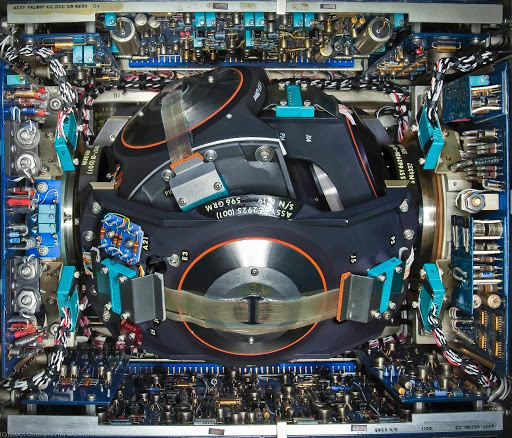
\includegraphics[height=0.8\linewidth]{Figures/INS_Concorde.jpg}
  \captionof{figure}{Physical INS System Used in Concorde}
  \label{fig:concordeINS}
\end{minipage}%
\begin{minipage}{.6\textwidth}
  \centering
  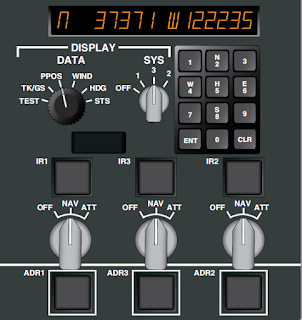
\includegraphics[height=0.8\linewidth]{Figures/INS-IRS_InterfacePanel.png}
  \captionof{figure}{Airbus INS Interface Panel Illustration}
  \label{fig:InterfaceINS}
\end{minipage}
\end{figure}

\vspace{5mm}
\noindent INS was a big leap in aircraft navigation. Around 1960s to 1990s, navigation reliability was a challenged for international flight around a higher earth latitude \cite{1964InertialNavigation}. The higher earth's latitude is the minimum region of compass accuracy and ground-based navigation aids (tower, etc) which made the navigation system unreliable. At this time, independent navigation was needed to overcome the challenge and INS was the solution.\\

\noindent Despite its accuracy and independence, INS build its error over its usage time. For instance, a tactical grade INS gain positional error up to 20 nautical miles per hour with gyroscope drift up to 10 deg per hour which is not reliable for a long-range navigation use. Therefore, in modern navigation system, integrating another type of navigation system (such as GPS) is proven to aid these issues.

\subsubsection{Submarine Navigation}
Before the INS became small and light, INS was broadly use for submarine navigation system or known as Ship Inertial Navigation System (SINS) \cite{NATOSINS}. The same concept applies where INS uses acceleration measurement to calculate the submarines' latitude, longitude, heading, and altitude given the initial referencing point.  One of the example of INS application in submarine is U.S.S Alabama, where INS is integrated vis Central Navigation Computer (CNC) with TRANSIT, LORAN-C, and SONAR for its overall navigation purposes \cite{HowNavigation}. Figure \ref{fig:USS_INS} shows the illustration of U.S.S Alabama navigation system.\\

\noindent It is important for a military submersible embeds an INS without any dependency from any other navigation aid. However, the objective of submarine design is to be able to travel in stealth mode where navigation which transmit waves such as GPS and sonar are not allowed \cite{Rogobete2018UsingPositioning}. For a long range movement, the INS alone could build an error and another navigation aid is required. To overcome this challenge, Kalman filter with Second Gradient of Gravity Field (SGG) sensor is required to allow continuous correction which improves the navigation accuracy an minimising INS drift. Simplified diagram of these scheme is shown on figure \ref{fig:INS_KALMAN}.\\

\noindent It is worth to be noted that in modern development, INS applications with other navigational aid is also used in autonomous submerged vehicles for research and military purposes.

\begin{figure}[!ht]
    \centering
    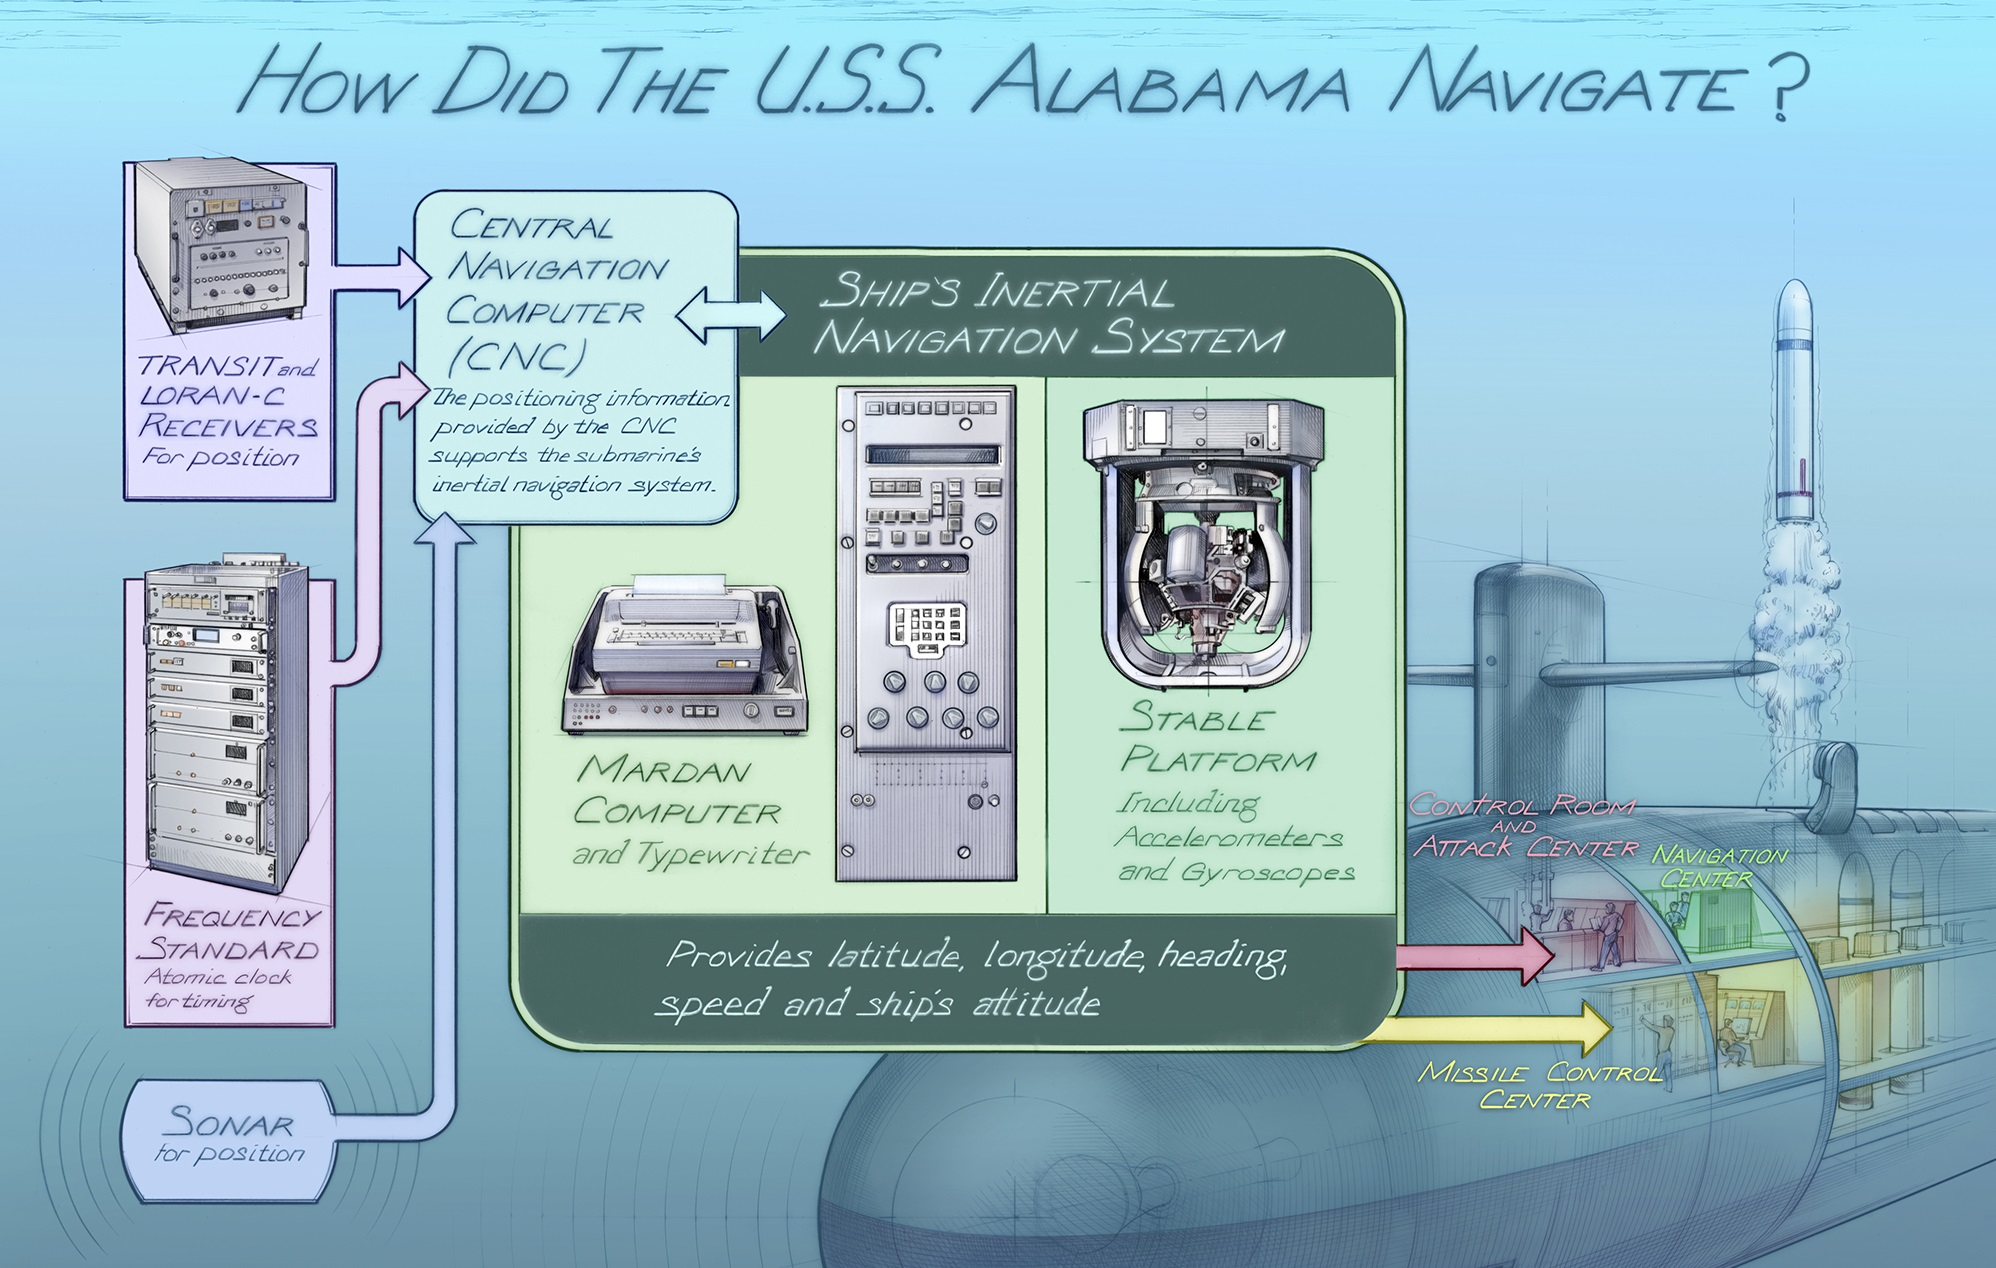
\includegraphics[scale=0.5]{Figures/USS_Alabama_INS.jpg}
    \caption{Simplified diagram of USS Alabama INS Navigation System \cite{HowNavigation}. }
    \label{fig:USS_INS}
    \vspace{2mm}
    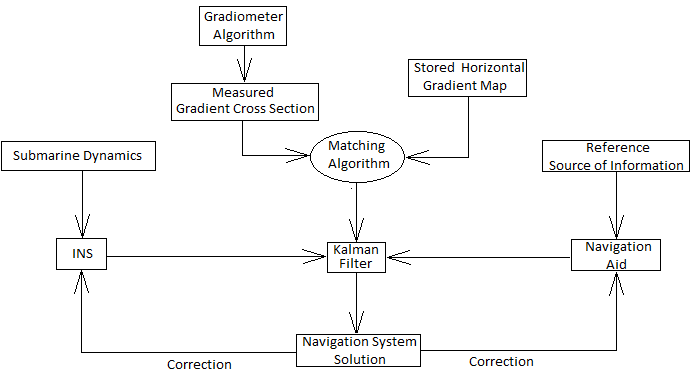
\includegraphics[scale=0.7]{Figures/INS Scheme KALMAN filter.png}
    \caption{INS Diagram correlated to Kalman filter with navigation aid and matching algorithm to improve drift correction \cite{Rogobete2018UsingPositioning}. }
    \label{fig:INS_KALMAN}
\end{figure}

\vspace{3cm}


\subsection{Enhanced Long Range Navigation (E-LORAN)}

%definition, basic system, difference between normal loran

%
\subsubsection{Telecommunication}

\subsubsection{Transportation Navigation}